\documentclass[11pt]{article}

\usepackage[margin=1in]{geometry}
\usepackage{amsmath,amssymb,amsfonts,bm}
\usepackage{graphicx}
\usepackage{xcolor}
\usepackage{float}
\usepackage{listings}
\usepackage{enumitem}
\usepackage{booktabs}
\usepackage{hyperref}
\usepackage{xurl}
\usepackage{fancyhdr}
\usepackage{tcolorbox}

\Urlmuskip=0mu plus 1mu
\hypersetup{
	breaklinks=true,
	colorlinks=true,
	linkcolor=blue,
	urlcolor=blue
}

\lstdefinestyle{matlabstyle}{
	language=Python,
	basicstyle=\ttfamily\small,
	frame=single,
	columns=fullflexible,
	showstringspaces=false,
}

\pagestyle{fancy}
\fancyhf{}
\fancyhead[L]{April 11, 2026}
\fancyhead[C]{Homework \#6: Image Classification}
\fancyhead[R]{Scott Nguyen}
\fancyfoot[C]{\thepage}

\begin{document}
	
	\section*{Homework \#6: Image Classification}
	April 11, 2026
	
	\section*{1 \quad Grading}
	
	You will receive zero credit if your answers appear to be AI-generated. During grading, I will try to assess your understanding of the material as opposed to text that appears to be AI-generated. On the other hand, consulting online sources or using AI-generated code to improve your understanding is expected.
	
	During the final exam, I will primarily focus on interpreting diagrams and figures that would be difficult to answer using AI-generated text. During the oral project, I will ask questions directly related to the material I ask in the homework. The credit is equally distributed among the problems.
	
	The classification examples are taken from:
	
	\url{https://github.com/ageron/handson-mlp/blob/main/03_classification.ipynb}
	
	\section*{2 \quad Problems}
	
	\subsection*{Problem 1. Selecting operating points and a sequential neural network structure}
	
	Consider the following two-stage classification system:
	
	\begin{itemize}
		\item Apply Object Detection to select possible objects.
		\item Classify extracted objects.
	\end{itemize}
	
	In this approach, the object detector should be fast and simple and readily available.
	
	\textbf{1(a)} We want to select an appropriate ROC point for the object detector.
	
	\begin{enumerate}[label=\roman*.]
		\item What is the ideal value?
		\item Can we accept a non-ideal value? Why?
		\item If we can accept a non-ideal value, what will this value be?
		\item Give the ideal ROC graph with the perfect operating point.
		\item Give the minimal ROC graph with random classification discussed in class.
		\item Give a realistic ROC graph with a non-ideal point that could work.
	\end{enumerate}
	
	\textbf{Solution}
	
	\begin{enumerate}[label=\roman*.]
		
		\item The ideal operating point is the perfect classifier:
		\[
		\text{Sensitivity} = 1, \qquad \text{Specificity} = 1.
		\]
		Since the ROC graph plots \(\text{Sensitivity}\) versus \(1-\text{Specificity}\), the ideal operating point is
		\[
		(0,1).
		\]
		
		\item Yes, a non-ideal value can be accepted. In this two-stage system, the detector only needs to pass possible objects to the next stage. Some false positives can be tolerated because the classifier can reject them later, but false negatives are more harmful because they remove true objects before classification.
		
		\item A suitable non-ideal operating point is one with very high sensitivity and low false positive rate. From the ROC point of view, we want the operating point as far to the left as possible while staying near the top. In other words, we want to drive false positives toward zero, since this moves the ROC curve to the left.
		
		\item The ideal ROC graph is shown in Figure~\ref{fig:ideal_roc}. Its start-point and end-point remain fixed at \((0,0)\) and \((1,1)\). The ideal curve goes vertically from \((0,0)\) to \((0,1)\), then horizontally from \((0,1)\) to \((1,1)\). The perfect operating point is at \((0,1)\).
		
		\begin{figure}[H]
			\centering
			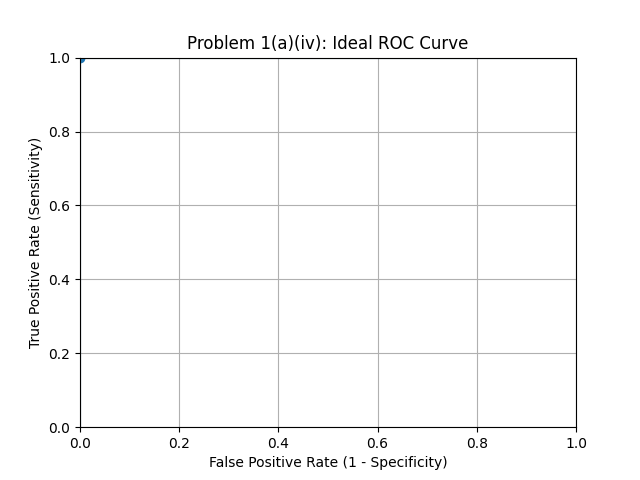
\includegraphics[width=0.5\textwidth]{plots/1a_iv_ideal_roc.png}
			\caption{Problem 1(a)(iv): Ideal ROC Curve}
			\label{fig:ideal_roc}
		\end{figure}
		
		\item The minimal ROC graph corresponding to random classification is shown in Figure~\ref{fig:random_roc}. Its start-point and end-point are also fixed at \((0,0)\) and \((1,1)\). The curve is the diagonal line from \((0,0)\) to \((1,1)\).
		
		\begin{figure}[H]
			\centering
			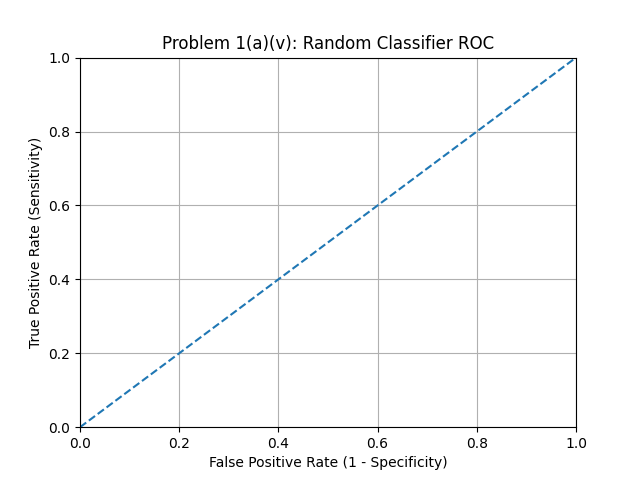
\includegraphics[width=0.5\textwidth]{plots/1a_v_random_roc.png}
			\caption{Problem 1(a)(v): Random Classifier ROC}
			\label{fig:random_roc}
		\end{figure}
		
		\item A realistic ROC graph with a non-ideal operating point is shown in Figure~\ref{fig:realistic_roc}. The start-point and end-point remain fixed, but compared to random classification, the curve is pushed upward and to the left. A useful operating point is near the top-left corner, since reducing false positives moves the ROC curve to the left while maintaining high sensitivity.
		
		\begin{figure}[H]
			\centering
			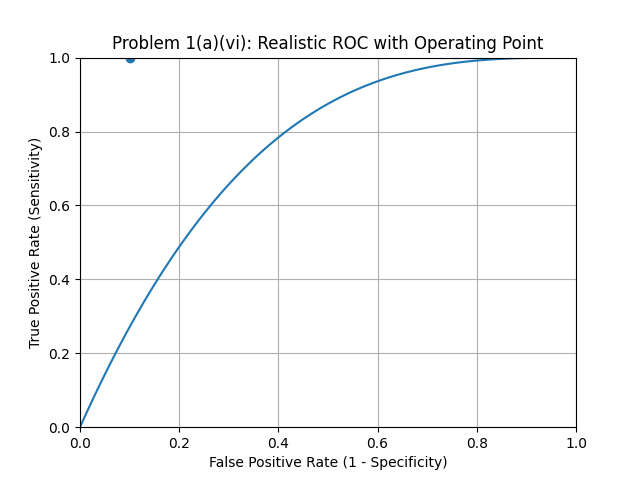
\includegraphics[width=0.5\textwidth]{plots/1a_vi_realistic_roc.png}
			\caption{Problem 1(a)(vi): Realistic ROC Curve with Operating Point}
			\label{fig:realistic_roc}
		\end{figure}
		
	\end{enumerate}
	
	\textbf{1(b)}  A common mistake is to use cross-validation to train each classifier separately and then take the optimized
	classifiers, put them together into the combined system, and report accuracy on the cross-validated combined system.
	Explain why this approach is wrong and why it tends to over-estimate classification accuracy. Here, you need to think in terms of the separation of the training and testing datasets.\\
	
	\textbf{Solution}
	
	This overestimates accuracy because the two stages are not independent. The second classifier depends on the outputs of the first, but separate cross-validation ignores the errors from the first stage. As a result, error propagation is not captured and the overall performance appears better than it actually is.
	
	\textbf{1(c)} Suggest a correction to 1(b). How would you properly estimate the accuracy of the full system?\\
	
	\textbf{Solution}
	
	The correct approach is to evaluate the entire pipeline together. Perform cross-validation on the full system by training both stages on the training split and then passing the test split through the detector and classifier sequentially. This includes the errors from the first stage and gives a more accurate estimate of full system performance.
	
	\textbf{1(d)} Sequential neural networks consist of several layers with nodes in each one. We can think of each node and its
	activation function as a detector. When the input to the activation function is positive, the neuron is said to fire.
	When the input to the activation function is negative, the neuron tries to ignore the input. In what follows, suppose
	that the neurons are arranged in a rectangular pattern that corresponds to the input image.
	Often, the number of nodes decreases with each sequential layer. Based on the discussions in this problem, answer
	the following:
	
	\begin{enumerate}[label=\roman*.]
		\item Suppose that we have a layer where no node is firing. What is the output?
		\item Suppose that we have a layer where every node is firing. What can we say about the layers below it?
		\item Suppose that you find that some nodes are firing but they are far from where your target object is. Will this
		work? Why or why not?
		\item Suppose that you find that some nodes are firing close to where your target object is. Will this work? Why or
		why not?
		\item Explain why using more nodes may increase the possibility of getting the ideal performance.
	\end{enumerate}
	
	\textbf{Solution}
	
	\begin{enumerate}[label=\roman*.]
		
		\item If no node is firing, the output is negative (no object detected), since there is no activation indicating the presence of the object.
		
		\item If all nodes are firing, it implies the system is over-activating and cannot discriminate between object and background, leading to many false positives.
		
		\item Nodes firing far from the object will not work well, since they do not correspond to the true object location and will increase false detections.
		
		\item Nodes firing near the object will work well, since they correctly respond to relevant features and help localize the object.
		
		\item More nodes improve performance because they provide better spatial coverage and allow the system to capture more variations of the object, increasing robustness and accuracy.
		
	\end{enumerate}
	
	\textbf{1(e)} A common method to assess whether a neural network is using the right information is to look at the neurons
	that are firing and overlaying them over the input image. In this case, please address the following:
	
	\begin{enumerate}[label=\roman*.]
		\item Suppose that we find that the strongest responses come from neurons that are far away from the object that
		we are after. Explain why this is bad.
		\item Suppose that we find that the strongest responses come from neurons that are centered around the object that
		we are after. Explain why this is much better.
	\end{enumerate}
	
	\textbf{Solution}
	
	\begin{enumerate}[label=\roman*.]
		
		\item Strong responses far from the object are bad because they indicate the neuron is activating on irrelevant background features, leading to false positives and poor localization.
		
		\item Strong responses near the object are better because they indicate the neuron is detecting meaningful features associated with the object, improving detection accuracy and localization.
		
	\end{enumerate}
	
	\subsection*{Problem 2. Fitting data using training and validation curves}
	Review loss functions. A loss function aims to define a function that, when minimized, the system reaches an ideal
	performance. An example is the mean squared error used in defining regression methods.
	
	\textbf{2(a)} During training, we often use a single set of images for training and another set of images for validation. For
	each example, sketch a training loss curve that demonstrates that:
	
	\begin{enumerate}[label=\roman*.]
		\item The neural network performance is improving during training. Explain.
		\item The neural network is not improving during training. Explain.
		\item The neural network has reached ideal performance during training. Explain.
	\end{enumerate}
	
	\textbf{Solution}
	
	\begin{enumerate}[label=\roman*.]
		
		\item Improving performance: the training loss decreases over epochs, indicating the model is learning and performance is improving. The curve shows a downward trend.
		
		\begin{figure}[H]
			\centering
			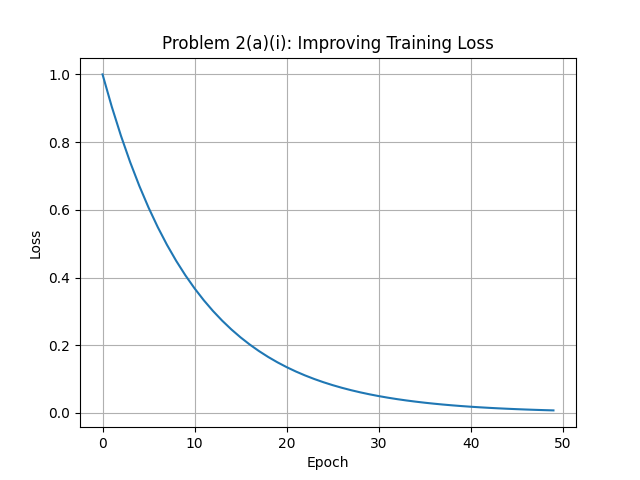
\includegraphics[width=0.45\textwidth]{plots/2a_i_improving.png}
			\caption{Problem 2(a)(i): Improving Training Loss}
		\end{figure}
		
		\item Not improving: the training loss remains approximately constant, indicating that the model is not learning or is stuck.
		
		\begin{figure}[H]
			\centering
			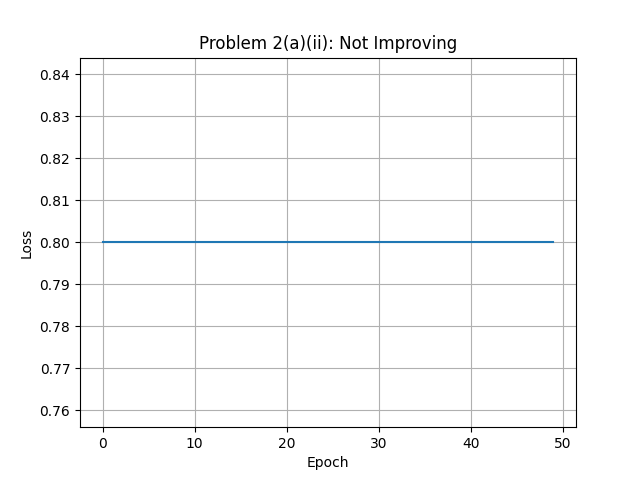
\includegraphics[width=0.45\textwidth]{plots/2a_ii_flat.png}
			\caption{Problem 2(a)(ii): Not Improving}
		\end{figure}
		
		\item Ideal performance reached: the training loss decreases and then levels off at a low value, indicating the model has converged.
		
		\begin{figure}[H]
			\centering
			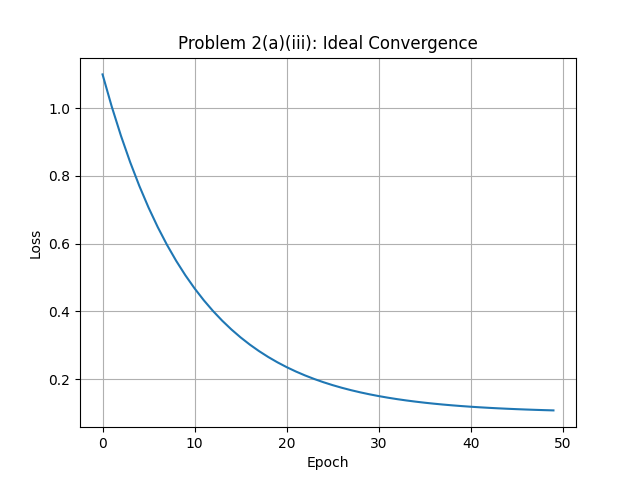
\includegraphics[width=0.45\textwidth]{plots/2a_iii_converged.png}
			\caption{Problem 2(a)(iii): Ideal Convergence}
		\end{figure}
		
	\end{enumerate}
	
	\textbf{2(b)} In order to understand how the example will generalize to new inputs, we look at the validation curve. For
	each example, sketch a validation loss curve that demonstrates that:
	
	\begin{enumerate}[label=\roman*.]
		\item The neural network is expected to perform well on unseen images. Explain.
		\item The validation loss curve follows an ideal trent. Explain.
		\item The validation loss curve follows the worst possible trend. Explain.
	\end{enumerate}
	
	\textbf{Solution}
	
	\begin{enumerate}[label=\roman*.]
		
		\item Good generalization: the validation loss decreases and stays close to the training loss, indicating the model generalizes well to unseen data.
		
		\begin{figure}[H]
			\centering
			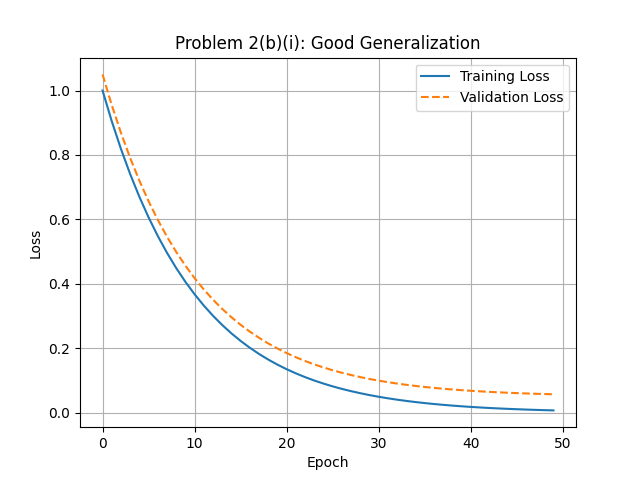
\includegraphics[width=0.45\textwidth]{plots/2b_i_good_generalization.png}
			\caption{Problem 2(b)(i): Good Generalization}
		\end{figure}
		
		\item Ideal trend: the validation loss decreases and then levels off at a low value, closely tracking the training loss, indicating good convergence and generalization.
		
		\begin{figure}[H]
			\centering
			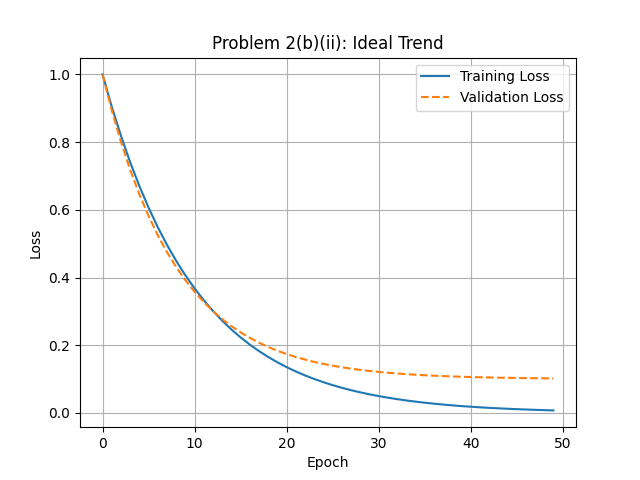
\includegraphics[width=0.45\textwidth]{plots/2b_ii_ideal.png}
			\caption{Problem 2(b)(ii): Ideal Trend}
		\end{figure}
		
		\item Worst trend: the validation loss increases while the training loss continues to decrease, indicating overfitting and poor generalization.
		
		\begin{figure}[H]
			\centering
			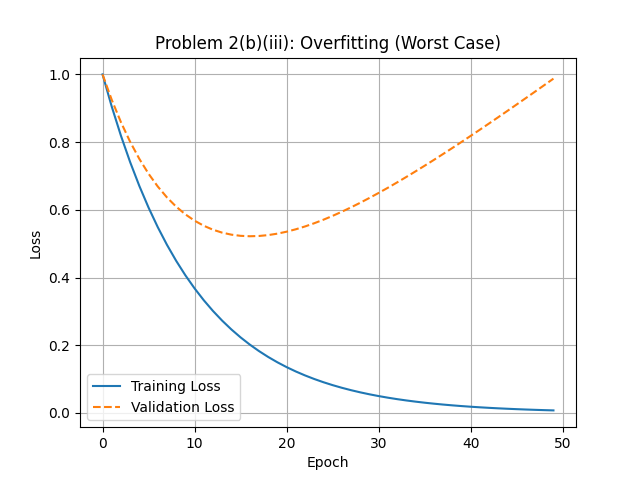
\includegraphics[width=0.45\textwidth]{plots/2b_iii_overfitting.png}
			\caption{Problem 2(b)(iii): Worst Trend}
		\end{figure}
		
	\end{enumerate}
	
	\textbf{2(c)} Assuming proper design of the training and validation datasets, we often study the relationship between the
	two curves to understand how to redesign our neural network. For each example, sketch a joint graph of the training
	and validation loss curves, identifying each curve to show:
	
	\begin{enumerate}[label=\roman*.]
		\item Ideal scenario. Explain.
		\item Overfitting. Explain.
		\item Underfitting. Explain.
		\item Good fitting. Explain.
	\end{enumerate}
	
	\textbf{Solution}
	
	\begin{enumerate}[label=\roman*.]
		
		\item Ideal: the training and validation losses both decrease and converge to low values, remaining very close to each other, indicating perfect generalization.
		
		\begin{figure}[H]
			\centering
			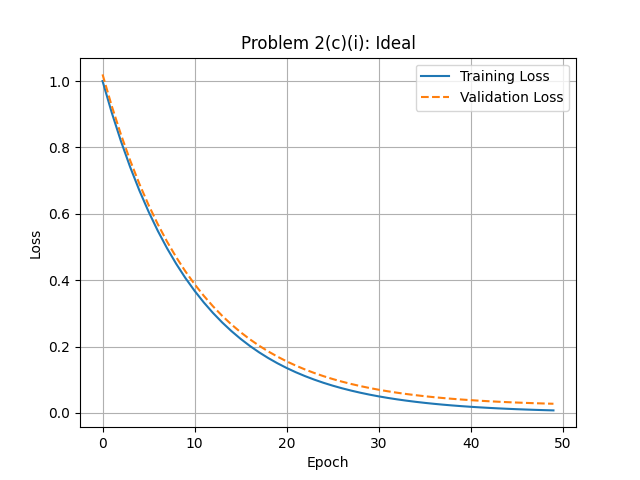
\includegraphics[width=0.45\textwidth]{plots/2c_i_ideal.png}
			\caption{Problem 2(c)(i): Ideal}
		\end{figure}
		
		\item Overfitting: the training loss continues to decrease, but the validation loss starts to increase, indicating the model is memorizing the training data and failing to generalize.
		
		\begin{figure}[H]
			\centering
			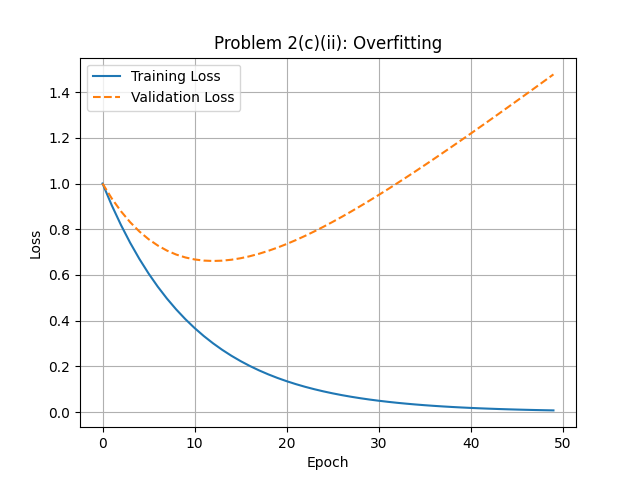
\includegraphics[width=0.45\textwidth]{plots/2c_ii_overfitting.png}
			\caption{Problem 2(c)(ii): Overfitting}
		\end{figure}
		
		\item Underfitting: both training and validation losses remain high and do not decrease significantly, indicating the model is too simple to capture the data.
		
		\begin{figure}[H]
			\centering
			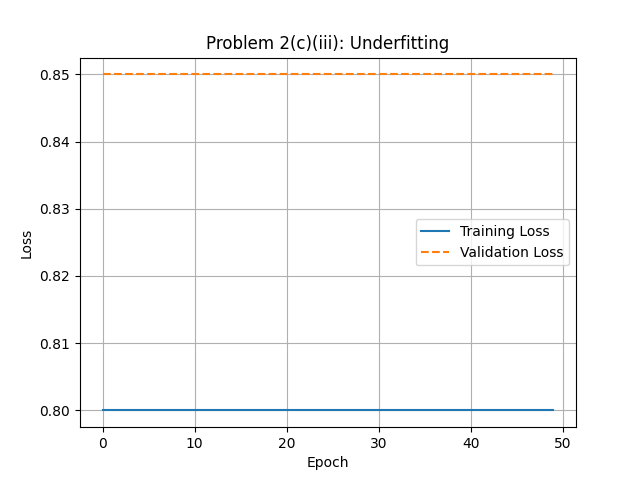
\includegraphics[width=0.45\textwidth]{plots/2c_iii_underfitting.png}
			\caption{Problem 2(c)(iii): Underfitting}
		\end{figure}
		
		\item Good fit: the training and validation losses both decrease and remain close, but the validation loss is slightly higher, indicating good generalization without overfitting.
		
		\begin{figure}[H]
			\centering
			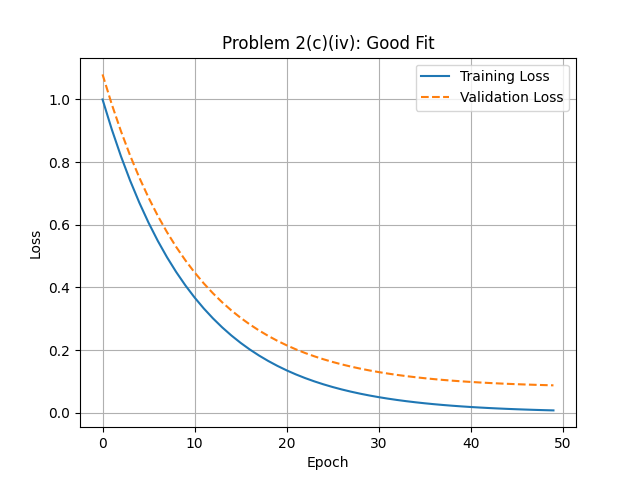
\includegraphics[width=0.45\textwidth]{plots/2c_iv_goodfit.png}
			\caption{Problem 2(c)(iv): Good Fit}
		\end{figure}
		
	\end{enumerate}
	
	\textbf{2(d)} For each of the following scenarios, provide at-least one strategy to address the problem:
	
	\begin{enumerate}[label=\roman*.]
		\item No learning is happening.
		\item The ability of the network to learn looks very bad.
		\item The network is underfitting.
		\item The network is overfitting.
		\item The network is fitting well but performance needs to be improved.
	\end{enumerate}
	
	\textbf{Solution}
	
	\begin{enumerate}[label=\roman*.]
		
		\item No learning: the model is not updating. This can be fixed by checking the implementation, learning rate, or data pipeline so that training actually progresses.
		
		\begin{figure}[H]
			\centering
			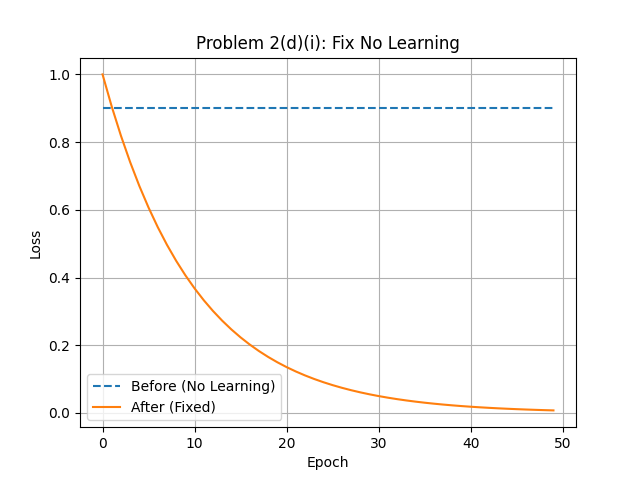
\includegraphics[width=0.45\textwidth]{plots/2d_i_fix_no_learning.png}
			\caption{Problem 2(d)(i): Fix No Learning}
		\end{figure}
		
		\item Poor learning: the model learns too slowly or ineffectively. This can be improved by tuning hyperparameters such as the learning rate, number of epochs, or initialization.
		
		\begin{figure}[H]
			\centering
			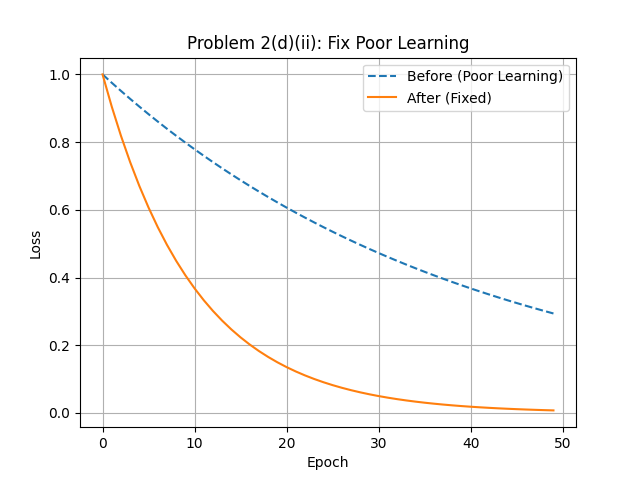
\includegraphics[width=0.45\textwidth]{plots/2d_ii_fix_poor_learning.png}
			\caption{Problem 2(d)(ii): Fix Poor Learning}
		\end{figure}
		
		\item Underfitting: the model is too simple to capture the data. This can be fixed by increasing model capacity, improving features, or training longer.
		
		\begin{figure}[H]
			\centering
			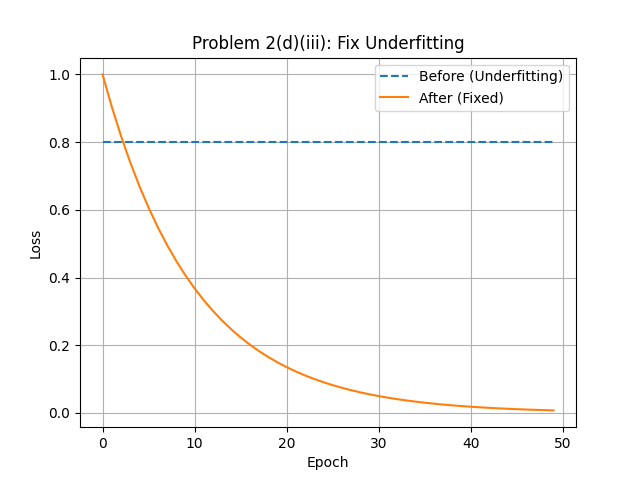
\includegraphics[width=0.45\textwidth]{plots/2d_iii_fix_underfitting.png}
			\caption{Problem 2(d)(iii): Fix Underfitting}
		\end{figure}
		
		\item Overfitting: the model memorizes the training data but does not generalize. This can be fixed using regularization, dropout, early stopping, or more data.
		
		\begin{figure}[H]
			\centering
			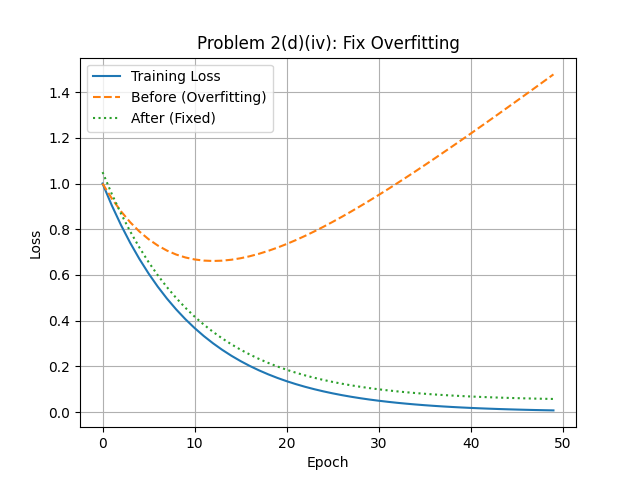
\includegraphics[width=0.45\textwidth]{plots/2d_iv_fix_overfitting.png}
			\caption{Problem 2(d)(iv): Fix Overfitting}
		\end{figure}
		
		\item Improve good model: when the model already performs well, improvements can be made by fine-tuning hyperparameters, improving data quality, or adding more data.
		
		\begin{figure}[H]
			\centering
			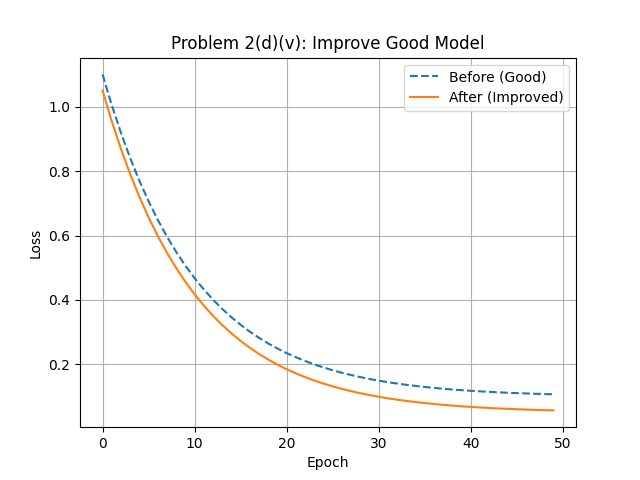
\includegraphics[width=0.45\textwidth]{plots/2d_v_improve_model.png}
			\caption{Problem 2(d)(v): Improve Good Model}
		\end{figure}
		
	\end{enumerate}
	
	\subsection*{Problem 3} \textbf{Binary Classification and Operating Points 3(a) (Balanced Datasets)} We return to our
	handwritten digits dataset:
	
	
	Digits:
	\[
	0,1,2,3,4,5,6,7,8,9
	\]
	
	We want to consider a binary classification problem:\\
	
	True class: The digit is prime: 2, 3, 5, or 7.\\
	False class: The digit is non-prime: 0, 1, 4, 6, 8, or 9.\\
	
	We want to work with a balanced dataset. Thus, your first task is to create a balanced dataset that has an equal number of elements in the True and False class.
	
	\textbf{3(a)} There are many possible approaches for creating a balanced dataset. A possible implementation of a balanced dataset approach is to use sampling with replacement from the class with the minimum number of samples.\\
	
	Here is some code that follows this approach:

	\begin{lstlisting}[style=matlabstyle]
		count_a = len(a_vals)
		count_b = len(b_vals)
		
		target_count = max(count_a, count_b)
		
		if count_a < count_b:
		a_sample = np.random.choice(a_vals, target_count, replace=True)
		b_sample = np.random.choice(b_vals, target_count, replace=False)
		else:
		a_sample = np.random.choice(a_vals, target_count, replace=False)
		b_sample = np.random.choice(b_vals, target_count, replace=True)
		
		balanced_samples = np.concatenate([a_sample, b_sample])
		np.random.shuffle(balanced_samples)
	\end{lstlisting}
	
	There is a problem with this approach. Use the code above to show how using this code to generate images that violate that the validation set should not contain any images seen during training.
	
	\textbf{Solution}
	
	The problem with this balancing approach is that sampling with replacement is done before splitting into training and validation sets. Because of this, the same original image can be selected multiple times. After shuffling and splitting, one copy of that image can appear in the training set while another copy appears in the validation set.
	
	Using the given approach, I obtained:
	\[
	\text{training samples} = 1721, \qquad
	\text{validation samples} = 431,
	\]
	and the number of leaked original images was
	\[
	131.
	\]
	
	Since the intersection between the training indices and validation indices is nonempty, this shows that some original images appear in both sets. Therefore, this method violates the requirement that the validation set should not contain images seen during training. This creates data leakage and can make the validation accuracy look better than it really is.
	
	\textbf{3(b)} Our second approach is to create a balanced dataset by sampling the larger class with the number of samples given by the smaller class.\\
	
	For this part, you are asked to provide:
	
	\begin{enumerate}[label=\roman*.]
		\item Provide the full Python code that creates a balanced dataset array for this problem.
		
		\item Print the first 10 elements of your array to show that it has been randomly shuffled.
		
		\item Print the length of the two classes to show that they are equal.
	\end{enumerate}
	
	\textbf{Solution}
	
	\begin{enumerate}[label=\roman*.]
		
		\item The balanced dataset was created by downsampling the larger class to match the size of the smaller class without replacement, then combining and shuffling the indices. This produces a balanced dataset array for the binary classification problem.
		
		\item The first 10 elements of the shuffled balanced dataset are:
		\[
		[1744,\ 65,\ 1785,\ 1463,\ 440,\ 1473,\ 178,\ 484,\ 400,\ 689]
		\]
		This shows that the array has been randomly shuffled.
		
		\item The number of samples in each class is:
		\[
		\text{True samples} = 721, \qquad \text{False samples} = 721.
		\]
		Since the two class sizes are equal, the dataset is balanced.
		
	\end{enumerate}
	
	\textbf{3(c)} \textbf{(Training and testing datasets)}. Based on the final length of your array in 3(b), you decide to use 80\%//
	
	For this part, you are asked to provide:
	
	\begin{enumerate}[label=\roman*.]
		\item Provide the full Python code that creates the training and testing arrays.
		
		\item Print the number of elements in all of the training set and testing set arrays.
		
		\item Print the shapes of each one of your arrays and explain what each dimension represents.
	\end{enumerate}
	
	\textbf{Solution}
	
	\begin{enumerate}[label=\roman*.]
		
		\item The training and testing arrays were created by splitting the balanced dataset into 80\% training and 20\% testing, then extracting the corresponding data and labels.
		
		\item The number of elements in each set is shown below:
		\begin{lstlisting}[style=matlabstyle]
			number of training samples: 1153
			number of testing samples: 289
		\end{lstlisting}
		
		\item The shapes of the arrays are:
		\begin{lstlisting}[style=matlabstyle]
			X_train shape: (1153, 64)
			y_train shape: (1153,)
			X_test shape: (289, 64)
			y_test shape: (289,)
		\end{lstlisting}
		
		For $X$, the first dimension is the number of samples and the second is the number of features (64 from the $8 \times 8$ image).  
		For $y$, the dimension represents the label for each sample.
		
	\end{enumerate}
	
	\textbf{3(d)} \textbf{(Testing Metrics)}. Write a function that accepts the predictions and ground truth and computes the following
	metrics:
	
	\begin{enumerate}[label=\roman*.]
		\item AUC: this is an excellent metric for looking at the performance of a classifier at all operating points.
		
		\item F1 score: a balanced metric for a single operating point.
		
		\item Confusion matrix: an all-encompassing matrix that captures performance for a single operating point.
		
		\item Classification accuracy.
		
		\item Precision and recall for a single operating point.
		
		\item Sensitivity and specificity for a single operating point.
	\end{enumerate}
	
	For full credit, you need to provide Python code for the function. Clearly identify the inputs to your function.
	
	\textbf{Solution}
	
	The function takes the following inputs:
	\begin{itemize}
		\item $y_{\text{true}}$: ground-truth binary labels
		\item $y_{\text{pred}}$: predicted binary labels at a chosen operating point
		\item $y_{\text{score}}$: predicted probabilities for the positive class
	\end{itemize}
	
	\begin{lstlisting}[style=matlabstyle]
		import numpy as np
		from sklearn.metrics import (
		roc_auc_score,
		f1_score,
		confusion_matrix,
		accuracy_score,
		precision_score,
		recall_score
		)
		
		def compute_metrics(y_true, y_pred, y_score):
		
		tn, fp, fn, tp = confusion_matrix(y_true, y_pred).ravel()
		
		auc = roc_auc_score(y_true, y_score)
		f1 = f1_score(y_true, y_pred)
		acc = accuracy_score(y_true, y_pred)
		precision = precision_score(y_true, y_pred)
		recall = recall_score(y_true, y_pred)
		
		sensitivity = tp / (tp + fn) if (tp + fn) > 0 else 0.0
		specificity = tn / (tn + fp) if (tn + fp) > 0 else 0.0
		
		return {
			"AUC": auc,
			"F1 Score": f1,
			"Confusion Matrix": np.array([[tn, fp], [fn, tp]]),
			"Accuracy": acc,
			"Precision": precision,
			"Recall": recall,
			"Sensitivity": sensitivity,
			"Specificity": specificity
		}
	\end{lstlisting}
	
	The computed metrics for the testing set are shown below:
	
	\begin{lstlisting}[style=matlabstyle]
		Inputs to compute_metrics:
		y_true shape: (289,)
		y_pred shape: (289,)
		y_score shape: (289,)
		
		AUC:
		0.9850488786659
		
		F1 Score:
		0.95
		
		Confusion Matrix:
		[[142   6]
		[  8 133]]
		
		Accuracy:
		0.9515570934256056
		
		Precision:
		0.9568345323741008
		
		Recall:
		0.9432624113475178
		
		Sensitivity:
		0.9432624113475178
		
		Specificity:
		0.9594594594594594
	\end{lstlisting}
	
	\textbf{3(e)} \textbf{(Cross-validation over the training set)}. Use your balanced training dataset from 3(c) to implement 5-fold
	cross-validation and print out the metrics for each fold. Here, you want to modify the example given below:
	
	\begin{lstlisting}[style=matlabstyle]
	from sklearn.model_selection import StratifiedKFold
	from sklearn.base import clone
				
	skfolds = StratifiedKFold(n_splits=3, random_state=42)
				
	for train_index, test_index in skfolds.split(X_train, y_train_5):
		clone_clf = clone(sgd_clf)
		X_train_folds = X_train[train_index]
		y_train_folds = y_train_5[train_index]
		X_test_fold = X_train[test_index]
		y_test_fold = y_train_5[test_index]
		
		clone_clf.fit(X_train_folds, y_train_folds)
		y_pred = clone_clf.predict(X_test_fold)
		n_correct = sum(y_pred == y_test_fold)
		print(n_correct / len(y_pred))
	\end{lstlisting}
	
	Instead of using Stochastic Gradient Descent, use the Random Forest Classifier.\\\\
	
	Please discuss the following:
	
	\begin{enumerate}[label=\roman*.]
		\item Are the folds using balanced datasets? Print the number of elements in each class to verify.
		
		\item We need to understand the variation among the folds
			\begin{enumerate}
				\item List the metrics for the highest AUC that you can achieve.
				\item List the metrics for the lowest AUC that you can achieve.
				\item Investigate the percentage variation between each metric’s minimum and maximum values. Is the variation
				reasonable?
			\end{enumerate}
	\end{enumerate}
	
	Note: An attractive feature of the Random Forest Classifier is that it can support explainable models. See	te2rules for details. It also allows us to assign Feature importance.\\
	
	\textbf{Solution}
	
	The following code uses 5-fold stratified cross-validation on the balanced training set from 3(c), replaces SGD with a Random Forest Classifier, and prints the metrics for each fold.
	
	\begin{lstlisting}[style=matlabstyle]
	from sklearn.model_selection import StratifiedKFold
	from sklearn.ensemble import RandomForestClassifier
	from sklearn.base import clone
	import numpy as np
		
	rf_clf = RandomForestClassifier(
		n_estimators=100,
		random_state=42
		)
		
	skfolds = StratifiedKFold(n_splits=5, shuffle=True, random_state=42)
		
	fold_results = []
		
	for fold_num, (cv_train_index, cv_test_index) in enumerate(
		skfolds.split(X_train, y_train_bin), start=1
		):
		print(f"========== Fold {fold_num} ==========")
		
		X_train_folds = X_train[cv_train_index]
		y_train_folds = y_train_bin[cv_train_index]
		
		X_test_fold = X_train[cv_test_index]
		y_test_fold = y_train_bin[cv_test_index]
		
		train_true_count = np.sum(y_train_folds == 1)
		train_false_count = np.sum(y_train_folds == 0)
		test_true_count = np.sum(y_test_fold == 1)
		test_false_count = np.sum(y_test_fold == 0)
		
		print("Training fold class counts:")
		print("  True :", train_true_count)
		print("  False:", train_false_count)
		
		print("Validation fold class counts:")
		print("  True :", test_true_count)
		print("  False:", test_false_count)
		
		clone_clf = clone(rf_clf)
		clone_clf.fit(X_train_folds, y_train_folds)
		
		y_score_fold = clone_clf.predict_proba(X_test_fold)[:, 1]
		y_pred_fold = (y_score_fold >= 0.5).astype(int)
		
		metrics = compute_metrics(y_test_fold, y_pred_fold, y_score_fold)
		
		print("Metrics:")
		for key, value in metrics.items():
		print(f"{key}:")
		print(value)
		print()
		
		fold_results.append({
			"fold": fold_num,
			"train_true": train_true_count,
			"train_false": train_false_count,
			"test_true": test_true_count,
			"test_false": test_false_count,
			"metrics": metrics
		})
		
		best_fold = max(fold_results, key=lambda r: r["metrics"]["AUC"])
		worst_fold = min(fold_results, key=lambda r: r["metrics"]["AUC"])
	\end{lstlisting}
	
	\begin{enumerate}[label=\roman*.]
		
		\item \textbf{Are the folds using balanced datasets?}
		
		The folds are \emph{approximately balanced}, but not perfectly equal. Since stratified cross-validation preserves class proportions, each fold keeps nearly the same ratio of the two classes. For example, the printed fold counts were:
		
		\begin{lstlisting}[style=matlabstyle]
			Fold 3
			Training fold class counts:
			True : 464
			False: 458
			Validation fold class counts:
			True : 116
			False: 115
			
			Fold 4
			Training fold class counts:
			True : 464
			False: 459
			Validation fold class counts:
			True : 116
			False: 114
			
			Fold 5
			Training fold class counts:
			True : 464
			False: 459
			Validation fold class counts:
			True : 116
			False: 114
		\end{lstlisting}
		
		So the folds are well balanced, even though they are not exactly equal in every split.
		
		\item \textbf{Variation among the folds}
		
		\begin{enumerate}
			
			\item \textbf{Metrics for the highest AUC}
			
			\begin{lstlisting}[style=matlabstyle]
				========== Highest AUC Fold ==========
				Fold: 5
				AUC:
				0.9970130066545675
				F1 Score:
				0.9694323144104804
				Confusion Matrix:
				[[112   2]
				[  5 111]]
				Accuracy:
				0.9695652173913043
				Precision:
				0.9823008849557522
				Recall:
				0.9568965517241379
				Sensitivity:
				0.9568965517241379
				Specificity:
				0.9824561403508771
			\end{lstlisting}
			
			\item \textbf{Metrics for the lowest AUC}
			
			\begin{lstlisting}[style=matlabstyle]
				========== Lowest AUC Fold ==========
				Fold: 3
				AUC:
				0.9943403298350825
				F1 Score:
				0.9655172413793104
				Confusion Matrix:
				[[111   4]
				[  4 112]]
				Accuracy:
				0.9653679653679653
				Precision:
				0.9655172413793104
				Recall:
				0.9655172413793104
				Sensitivity:
				0.9655172413793104
				Specificity:
				0.9652173913043478
			\end{lstlisting}
			
			\item \textbf{Percentage variation between minimum and maximum values}
			
			\begin{lstlisting}[style=matlabstyle]
				========== Percentage Variation ==========
				AUC
				min: 0.9943403298350825
				max: 0.9970130066545675
				percent variation: 0.26878893868543985
				
				F1 Score
				min: 0.946058091286307
				max: 0.9785407725321889
				percent variation: 3.43347639484979
				
				Accuracy
				min: 0.9434782608695652
				max: 0.9783549783549783
				percent variation: 3.6966106090530015
				
				Precision
				min: 0.912
				max: 0.9823008849557522
				percent variation: 7.70843036795528
				
				Recall
				min: 0.9568965517241379
				max: 0.9827586206896551
				percent variation: 2.702702702702702
				
				Sensitivity
				min: 0.9568965517241379
				max: 0.9827586206896551
				percent variation: 2.702702702702702
				
				Specificity
				min: 0.9035087719298246
				max: 0.9824561403508771
				percent variation: 8.737864077669894
			\end{lstlisting}
			
			The variation is reasonable overall. The AUC varies by only about \(0.27\%\), which shows that the classifier is very stable across folds. F1 score and accuracy also vary only by about \(3\%-4\%\), which is still small. Precision and specificity have somewhat larger variation, but both remain high, so the Random Forest still performs consistently well across the different folds.
			
		\end{enumerate}
		
	\end{enumerate}
	
	\textbf{3(f)} \textbf{(parameter optimization using GridSearchCV()} and final results on the test set) In practice, cross-validation is primarily used for optimizing the classifier over the training set. The most advanced examples can be found at model selection using Scikit Learn. Here, we just want to study a simple example by finding the optimal number of trees and the optimal depth of each tree. Then, we want to report the results on our test set.\\
	
	Here is some code to get you started (not fully verified):
	
	\begin{lstlisting}[style=matlabstyle]
		from sklearn . ensemble import RandomForestClassifier
		from sklearn . model_selection import GridSearchCV
		from sklearn . metrics import roc_auc_score , make_scorer
		from sklearn . datasets import make_classification
		from sklearn . model_selection import train_test_split
		
		# Define the R a n d o m F o r e s t C l a s s i f i e r
		rf = RandomForestClassifier ( random_state =42 )
		# Define the h y p e r p a r a m e t e r grid
		param_grid = {
			’ n_estimators ’: [100 , 200 , 500 ],
			’max_depth ’: [None , 10 , 20 , 30]
		}
		# Define the scorer based on AUC
		auc_scorer = make_scorer ( roc_auc_score , needs_proba = True )
		
		# Set up GridSearchCV
		grid_search = GridSearchCV ( estimator =rf ,
					param_grid = param_grid ,
					scoring = auc_scorer ,
					cv=5 , # 5- fold cross - validation
					n_jobs =-1 , # Use all available CPU cores
					verbose =2)
					
		# Run GridSearchCV
		grid_search . fit ( X_train , y_train )
		
		# Best parameters and best AUC score
		print (" Best parameters :", grid_search . best_params_ )
		print (" Best AUC score :", grid_search . best_score_ )
		
		# Evaluate on test set
		best_rf = grid_search . best_estimator_
		y_pred_proba = best_rf . predict_proba ( X_test )[:, 1]
		test_auc = roc_auc_score ( y_test , y_pred_proba )
		print (" Test AUC :", test_auc )
	\end{lstlisting}
	
	Modify the code for our problem. For full credit, you need to provide:
	
	\begin{enumerate}[label=\roman*.]
		\item Working Python code.
		\item All of the metrics were evaluated over the final test set.
		\item A discussion regarding the difference in values between what was achieved on the validation set and the final
		test set.
	\end{enumerate}
	
	\textbf{Solution}
	
	The following code uses \texttt{GridSearchCV} on the balanced training set to optimize the Random Forest Classifier over the number of trees and the maximum tree depth. The best model is then evaluated on the final test set.
	
		\begin{lstlisting}[style=matlabstyle]
			import numpy as np
			from sklearn.ensemble import RandomForestClassifier
			from sklearn.model_selection import GridSearchCV
			from sklearn.metrics import (
			roc_auc_score,
			f1_score,
			confusion_matrix,
			accuracy_score,
			precision_score,
			recall_score
			)
			
			def compute_metrics(y_true, y_pred, y_score):
			tn, fp, fn, tp = confusion_matrix(y_true, y_pred).ravel()
			
			auc = roc_auc_score(y_true, y_score)
			f1 = f1_score(y_true, y_pred)
			acc = accuracy_score(y_true, y_pred)
			precision = precision_score(y_true, y_pred)
			recall = recall_score(y_true, y_pred)
			
			sensitivity = tp / (tp + fn) if (tp + fn) > 0 else 0.0
			specificity = tn / (tn + fp) if (tn + fp) > 0 else 0.0
			
			return {
				"AUC": auc,
				"F1 Score": f1,
				"Confusion Matrix": np.array([[tn, fp], [fn, tp]]),
				"Accuracy": acc,
				"Precision": precision,
				"Recall": recall,
				"Sensitivity": sensitivity,
				"Specificity": specificity
			}
			
			y_binary = np.isin(y, [2, 3, 5, 7]).astype(int)
			y_train_bin = y_binary[train_idx]
			y_test_bin = y_binary[test_idx]
			
			rf = RandomForestClassifier(random_state=42)
			
			param_grid = {
				"n_estimators": [50, 100, 200, 500],
				"max_depth": [None, 5, 10, 20, 30]
			}
			
			grid_search = GridSearchCV(
			estimator=rf,
			param_grid=param_grid,
			scoring="roc_auc",
			cv=5,
			n_jobs=1,
			verbose=2
			)
			
			grid_search.fit(X_train, y_train_bin)
			
			print("Best parameters:", grid_search.best_params_)
			print("Best validation AUC:", grid_search.best_score_)
			
			best_rf = grid_search.best_estimator_
			
			y_test_score = best_rf.predict_proba(X_test)[:, 1]
			y_test_pred = (y_test_score >= 0.5).astype(int)
			
			test_metrics = compute_metrics(y_test_bin, y_test_pred, y_test_score)
			
			print("Final test-set metrics:")
			for key, value in test_metrics.items():
			print(f"{key}:")
			print(value)
			print()
			
			print("Validation vs Test AUC difference:")
			print("Validation AUC:", grid_search.best_score_)
			print("Test AUC:", test_metrics["AUC"])
			print("Absolute difference:", abs(grid_search.best_score_ - test_metrics["AUC"]))
		\end{lstlisting}
	
	\begin{enumerate}[label=\roman*.]
		
		\item \textbf{Working Python code}
		
		The code above performs hyperparameter optimization over the training set only, using 5-fold cross-validation and AUC as the scoring metric.
		
		\item \textbf{Final test-set metrics}
		
		The best hyperparameters found by grid search were:
		\begin{lstlisting}[style=matlabstyle]
			Best parameters: {'max_depth': None, 'n_estimators': 500}
			Best validation AUC: 0.9961051053420658
		\end{lstlisting}
		
		The final metrics on the test set were:
		\begin{lstlisting}[style=matlabstyle]
			Final test-set metrics:
			AUC:
			0.9948725321065747
			
			F1 Score:
			0.9619377162629758
			
			Confusion Matrix:
			[[139   9]
			[  2 139]]
			
			Accuracy:
			0.9619377162629758
			
			Precision:
			0.9391891891891891
			
			Recall:
			0.9858156028368794
			
			Sensitivity:
			0.9858156028368794
			
			Specificity:
			0.9391891891891891
		\end{lstlisting}
		
		\item \textbf{Discussion of validation vs. final test results}
		
		The validation AUC from cross-validation was:
		\begin{lstlisting}[style=matlabstyle]
			0.9961051053420658
		\end{lstlisting}
		
		The final test-set AUC was:
		\begin{lstlisting}[style=matlabstyle]
			0.9948725321065747
		\end{lstlisting}
		
		The absolute difference was:
		\begin{lstlisting}[style=matlabstyle]
			0.0012325732354910857
		\end{lstlisting}
		
		This difference is very small, which suggests that the model generalizes well from the validation folds to the final test set. In other words, the cross-validation estimate was a good predictor of final performance. The test AUC is slightly lower than the validation AUC, which is expected, since the final test set contains unseen data and usually gives a slightly more realistic estimate of performance.
		
	\end{enumerate}
	
	\subsection*{Problem 4} In this problem we want to design a multiclass classifier based on the MNIST dataset that determines
	whether a digit image belongs to: (i) Class A: 0, 1, 2, (ii) Class B: 3, 4, 5, and (iii) Class C: 6, 7, 8, 9. For this
	example, produce the confusion matrix for the Stochastic Gradient Descent classifier and show examples of (i) correct
	classification and (ii) incorrect classification.
	
	Confusion matrix + examples.
	
	\textbf{Solution}
	
	The multiclass labels were created from the original digit labels by defining:
	\begin{itemize}
		\item Class A \(= \{0,1,2\}\)
		\item Class B \(= \{3,4,5\}\)
		\item Class C \(= \{6,7,8,9\}\)
	\end{itemize}
	
	The following code creates the multiclass target array, trains a Stochastic Gradient Descent classifier, computes the confusion matrix, and saves one correctly classified and one incorrectly classified example.
	
	\begin{lstlisting}[style=matlabstyle]
	import os
	import numpy as np
	import matplotlib.pyplot as plt
			
	from sklearn.datasets import load_digits
	from sklearn.model_selection import train_test_split
	from sklearn.linear_model import SGDClassifier
	from sklearn.metrics import confusion_matrix
			
	os.makedirs("plots", exist_ok=True)
	np.random.seed(42)
			
	digits = load_digits()
	X = digits.data
	y = digits.target
			
	# 0 = Class A, 1 = Class B, 2 = Class C
	y_abc = np.zeros_like(y)
			
	mask_b = np.logical_or(np.logical_or(y == 3, y == 4), y == 5)
	mask_c = np.logical_or(np.logical_or(np.logical_or(y == 6, y == 7), y == 8), y == 9)
			
	y_abc[mask_b] = 1
	y_abc[mask_c] = 2
			
	X_train, X_test, y_train_abc, y_test_abc = train_test_split(
		X,
		y_abc,
		test_size=0.2,
		random_state=42,
		stratify=y_abc
		)
			
	sgd_clf = SGDClassifier(random_state=42, max_iter=1000, tol=1e-3)
	sgd_clf.fit(X_train, y_train_abc)
			
	y_pred_abc = sgd_clf.predict(X_test)
	cm = confusion_matrix(y_test_abc, y_pred_abc)
			
	print("Confusion Matrix:")
	print(cm)
			
	correct_idx = np.where(y_pred_abc == y_test_abc)[0][0]
	incorrect_candidates = np.where(y_pred_abc != y_test_abc)[0]
	incorrect_idx = incorrect_candidates[0] if len(incorrect_candidates) > 0 else None
			
	class_names = {
		0: "Class A",
		1: "Class B",
		2: "Class C"
		}
			
	print("Correct example:")
	print("Test index:", correct_idx)
	print("True label:", y_test_abc[correct_idx], "-", class_names[y_test_abc[correct_idx]])
	print("Predicted label:", y_pred_abc[correct_idx], "-", class_names[y_pred_abc[correct_idx]])
			
	print("Incorrect example:")
	print("Test index:", incorrect_idx)
	print("True label:", y_test_abc[incorrect_idx], "-", class_names[y_test_abc[incorrect_idx]])
	print("Predicted label:", y_pred_abc[incorrect_idx], "-", class_names[y_pred_abc[incorrect_idx]])
			
	plt.figure()
	plt.imshow(X_test[correct_idx].reshape(8, 8), cmap="gray")
	plt.title(
	f"Correct Example\nTrue: {class_names[y_test_abc[correct_idx]]}, "
	f"Pred: {class_names[y_pred_abc[correct_idx]]}"
		)
	plt.axis("off")
	plt.savefig("plots/problem4_correct_example.png")
	plt.close()
			
	plt.figure()
	plt.imshow(X_test[incorrect_idx].reshape(8, 8), cmap="gray")
	plt.title(
	f"Incorrect Example\nTrue: {class_names[y_test_abc[incorrect_idx]]}, "
	f"Pred: {class_names[y_pred_abc[incorrect_idx]]}"
			)
	plt.axis("off")
	plt.savefig("plots/problem4_incorrect_example.png")
	plt.close()
	\end{lstlisting}

	The class counts for the new multiclass target were:
	
	\begin{lstlisting}[style=matlabstyle]
		Class counts:
		Class A: 537
		Class B: 546
		Class C: 714
	\end{lstlisting}
	
	The confusion matrix for the SGD classifier was:
	
	\begin{lstlisting}[style=matlabstyle]
		[[106   1   1]
		[  9  80  20]
		[ 18  11 114]]
	\end{lstlisting}
	
	This confusion matrix shows that the classifier performs best on Class A and Class C, while Class B has more misclassifications, especially into Class C.
	
	An example of a correctly classified sample was:
	
	\begin{lstlisting}[style=matlabstyle]
		Correct example:
		Test index: 0
		True label: 2 - Class C
		Predicted label: 2 - Class C
	\end{lstlisting}
	
	An example of an incorrectly classified sample was:
	
	\begin{lstlisting}[style=matlabstyle]
		Incorrect example:
		Test index: 1
		True label: 1 - Class B
		Predicted label: 2 - Class C
	\end{lstlisting}
	
	The saved example images are shown in Figures~\ref{fig:problem4_correct} and~\ref{fig:problem4_incorrect}.
	
	\begin{figure}[H]
		\centering
		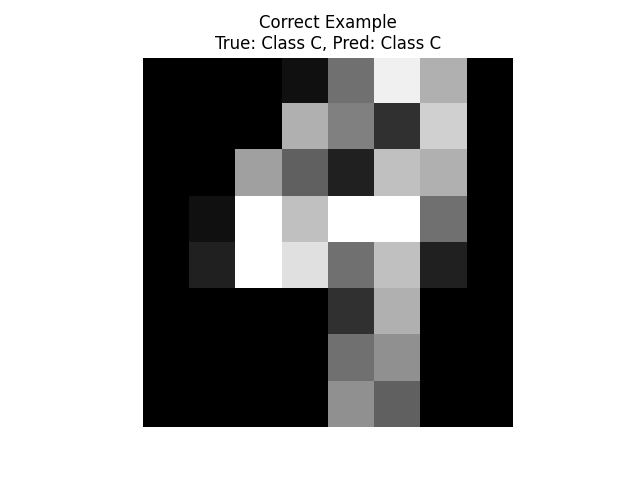
\includegraphics[width=0.35\textwidth]{plots/problem4_correct_example.png}
		\caption{Problem 4: Example of a correct classification}
		\label{fig:problem4_correct}
	\end{figure}
	
	\begin{figure}[H]
		\centering
		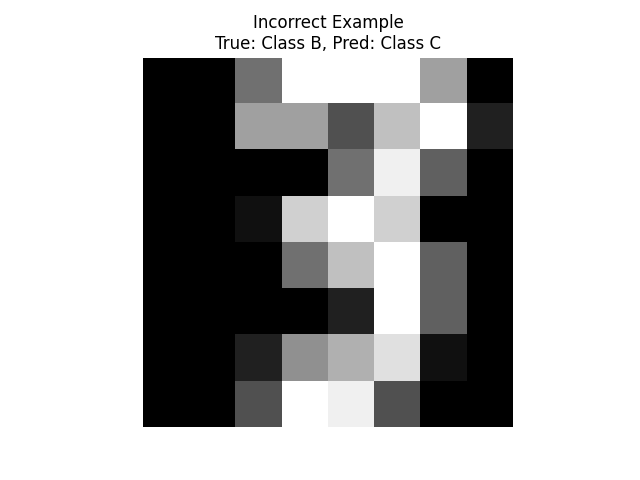
\includegraphics[width=0.35\textwidth]{plots/problem4_incorrect_example.png}
		\caption{Problem 4: Example of an incorrect classification}
		\label{fig:problem4_incorrect}
	\end{figure}

	\subsection*{Problem 5. Multiobjective Optimization}
	
	In this problem, you will select different operating points from the ROC curve. Use the example from \texttt{03\_classification.ipynb} of how to plot ROC curves to find the threshold for the following operating points:
	
	\begin{enumerate}[label=\roman*.]
		
		\item Maximize true-positive rate:
		\[
		\max_{\text{threshold}} \ \text{tpr} 
		\quad \text{subject to:} \quad \text{fpr} \leq 0.1.
		\]
		
		\item Minimize false-positive rate:
		\[
		\min_{\text{threshold}} \ \text{fpr} 
		\quad \text{subject to:} \quad \text{tpr} \geq 0.9.
		\]
		
		\item Balanced approach:
		\[
		\min_{\text{threshold}} \ \left(-\text{tpr} + 2 \cdot \text{fpr}\right)
		\quad \text{subject to:} \quad (\text{tpr} \geq 0.8) \ \text{and} \ (\text{fpr} \leq 0.1).
		\]
		
		\item For the balanced approach, why do we have a negative sign in front of tpr?
		
		\item For the balanced approach, what is the relationship with respect to the slope of the ROC curve?
		
	\end{enumerate}
	
	\textbf{Hint:} Take the derivative with respect to the threshold, set it to zero, and derive an expression with respect to the slope of the curve.
	
	\textbf{Solution}
	
	The following code trains a Random Forest classifier, computes the ROC curve, and identifies thresholds for the required operating points.

	\begin{lstlisting}[style=matlabstyle]
	import os
	import numpy as np
	import matplotlib.pyplot as plt
	
	from sklearn.datasets import load_digits
	from sklearn.model_selection import train_test_split
	from sklearn.ensemble import RandomForestClassifier
	from sklearn.metrics import (
	roc_curve,
	auc,
	confusion_matrix,
	f1_score,
	accuracy_score,
	precision_score,
	recall_score
	)
	
	# ---------------------------------------------------------
	# Problem 5: Multiobjective Optimization
	# ---------------------------------------------------------
	
	os.makedirs("plots", exist_ok=True)
	
	# load dataset
	digits = load_digits()
	X = digits.data
	y = digits.target
	
	# binary labels
	# positive (True): 2, 3, 5, 7
	# negative (False): 0, 1, 4, 6, 8, 9
	y_binary = np.isin(y, [2, 3, 5, 7]).astype(int)
	
	# train/test split
	X_train, X_test, y_train_bin, y_test_bin = train_test_split(
	X,
	y_binary,
	test_size=0.2,
	random_state=42,
	stratify=y_binary
	)
	
	# train classifier
	rf = RandomForestClassifier(
	n_estimators=500,
	max_depth=None,
	random_state=42
	)
	rf.fit(X_train, y_train_bin)
	
	# prediction scores
	y_score = rf.predict_proba(X_test)[:, 1]
	
	# ROC curve
	fpr, tpr, thresholds = roc_curve(y_test_bin, y_score)
	roc_auc = auc(fpr, tpr)
	
	# ---------------------------------------------------------
	# helper functions
	# ---------------------------------------------------------
	def compute_single_point_metrics(y_true, y_pred):
	tn, fp, fn, tp = confusion_matrix(y_true, y_pred).ravel()
	
	acc = accuracy_score(y_true, y_pred)
	f1 = f1_score(y_true, y_pred)
	precision = precision_score(y_true, y_pred, zero_division=0)
	recall = recall_score(y_true, y_pred, zero_division=0)
	
	sensitivity = tp / (tp + fn) if (tp + fn) > 0 else 0.0
	specificity = tn / (tn + fp) if (tn + fp) > 0 else 0.0
	
	return {
		"Confusion Matrix": np.array([[tn, fp], [fn, tp]]),
		"Accuracy": acc,
		"F1 Score": f1,
		"Precision": precision,
		"Recall": recall,
		"Sensitivity": sensitivity,
		"Specificity": specificity
	}
	
	def print_solution(name, idx):
	th = thresholds[idx]
	chosen_fpr = fpr[idx]
	chosen_tpr = tpr[idx]
	
	y_pred = (y_score >= th).astype(int)
	metrics = compute_single_point_metrics(y_test_bin, y_pred)
	
	print("==================================================")
	print(name)
	print("threshold:", th)
	print("fpr:", chosen_fpr)
	print("tpr:", chosen_tpr)
	for key, value in metrics.items():
	print(f"{key}:")
	print(value)
	print()
	
	# ---------------------------------------------------------
	# (i) maximize tpr subject to fpr <= 0.1
	# ---------------------------------------------------------
	valid_i = np.where(fpr <= 0.1)[0]
	idx_i = valid_i[np.argmax(tpr[valid_i])]
	
	# ---------------------------------------------------------
	# (ii) minimize fpr subject to tpr >= 0.9
	# ---------------------------------------------------------
	valid_ii = np.where(tpr >= 0.9)[0]
	idx_ii = valid_ii[np.argmin(fpr[valid_ii])]
	
	# ---------------------------------------------------------
	# (iii) balanced approach
	# minimize (-tpr + 2*fpr)
	# subject to (tpr >= 0.8) and (fpr <= 0.1)
	# ---------------------------------------------------------
	valid_iii = np.where((tpr >= 0.8) & (fpr <= 0.1))[0]
	objective_iii = -tpr[valid_iii] + 2.0 * fpr[valid_iii]
	idx_iii = valid_iii[np.argmin(objective_iii)]
	
	# ---------------------------------------------------------
	# print results
	# ---------------------------------------------------------
	print("ROC AUC:", roc_auc)
	print()
	
	print_solution("(i) Maximize tpr subject to fpr <= 0.1", idx_i)
	print_solution("(ii) Minimize fpr subject to tpr >= 0.9", idx_ii)
	print_solution("(iii) Balanced approach: minimize (-tpr + 2*fpr)", idx_iii)
	
	# ---------------------------------------------------------
	# (iv) explanation of negative sign
	# ---------------------------------------------------------
	print("==================================================")
	print("(iv) Why is there a negative sign in front of tpr?")
	print("Because we want to maximize tpr, but the optimization is written as a minimization problem.")
	print("Using -tpr converts maximizing tpr into minimizing -tpr.")
	print()
	
	# ---------------------------------------------------------
	# (v) slope relationship
	# For objective J = -tpr + 2*fpr
	# dJ/d(threshold) = -dtpr/dtau + 2*dfpr/dtau = 0
	# so dtpr/dfpr = 2
	# ---------------------------------------------------------
	print("==================================================")
	print("(v) Slope relationship for the balanced approach")
	print("For J = -tpr + 2*fpr, setting dJ/d(threshold) = 0 gives:")
	print("    -d(tpr)/d(threshold) + 2*d(fpr)/d(threshold) = 0")
	print("So:")
	print("    d(tpr)/d(fpr) = 2")
	print("Thus, the optimal point is related to a ROC slope of 2.")
	print()
	
	# ---------------------------------------------------------
	# plot ROC curve and selected operating points
	# ---------------------------------------------------------
	plt.figure()
	plt.plot(fpr, tpr, label=f"ROC curve (AUC = {roc_auc:.4f})")
	plt.scatter(fpr[idx_i], tpr[idx_i], label="(i) max tpr, fpr<=0.1")
	plt.scatter(fpr[idx_ii], tpr[idx_ii], label="(ii) min fpr, tpr>=0.9")
	plt.scatter(fpr[idx_iii], tpr[idx_iii], label="(iii) balanced")
	plt.xlabel("False Positive Rate")
	plt.ylabel("True Positive Rate")
	plt.title("Problem 5 ROC Operating Points")
	plt.legend()
	plt.grid()
	plt.savefig("plots/problem5_roc.png")
	plt.close()
	\end{lstlisting}
	
	The ROC AUC for the classifier was:
	
	\begin{lstlisting}[style=matlabstyle]
		ROC AUC: 0.998874742798354
	\end{lstlisting}
	
	\begin{enumerate}[label=\roman*.]
		
		\item \textbf{Maximize true-positive rate subject to $\text{fpr} \leq 0.1$}
		
		\begin{lstlisting}[style=matlabstyle]
			threshold: 0.352
			fpr: 0.06944444444444445
			tpr: 1.0
			
			Confusion Matrix:
			[[201  15]
			[  0 144]]
			
			Accuracy:
			0.9583333333333334
			
			F1 Score:
			0.9504950495049505
			
			Precision:
			0.9056603773584906
			
			Recall:
			1.0
			
			Sensitivity:
			1.0
			
			Specificity:
			0.9305555555555556
		\end{lstlisting}
		
		\item \textbf{Minimize false-positive rate subject to $\text{tpr} \geq 0.9$}
		
		\begin{lstlisting}[style=matlabstyle]
			threshold: 0.592
			fpr: 0.0
			tpr: 0.9722222222222222
			
			Confusion Matrix:
			[[216   0]
			[  4 140]]
			
			Accuracy:
			0.9888888888888889
			
			F1 Score:
			0.9859154929577465
			
			Precision:
			1.0
			
			Recall:
			0.9722222222222222
			
			Sensitivity:
			0.9722222222222222
			
			Specificity:
			1.0
		\end{lstlisting}
		
		\item \textbf{Balanced approach}
		
		\begin{lstlisting}[style=matlabstyle]
			threshold: 0.592
			fpr: 0.0
			tpr: 0.9722222222222222
			
			Confusion Matrix:
			[[216   0]
			[  4 140]]
			
			Accuracy:
			0.9888888888888889
			
			F1 Score:
			0.9859154929577465
			
			Precision:
			1.0
			
			Recall:
			0.9722222222222222
			
			Sensitivity:
			0.9722222222222222
			
			Specificity:
			1.0
		\end{lstlisting}
		
		\item \textbf{Why is there a negative sign in front of tpr?}
		
		\begin{lstlisting}[style=matlabstyle]
			Because we want to maximize tpr, but the optimization is written
			as a minimization problem. Using -tpr converts maximizing tpr
			into minimizing -tpr.
		\end{lstlisting}
		
		\item \textbf{Slope relationship}
		
		\begin{lstlisting}[style=matlabstyle]
			For J = -tpr + 2*fpr:
			
			-d(tpr)/d(threshold) + 2*d(fpr)/d(threshold) = 0
			
			=> d(tpr)/d(fpr) = 2
			
			So the optimal operating point corresponds to a ROC slope of 2.
		\end{lstlisting}
		
	\end{enumerate}
	
	The ROC curve was saved as:
	
	\begin{lstlisting}[style=matlabstyle]
		plots/problem5_roc.png
	\end{lstlisting}
	
	\begin{figure}[H]
		\centering
		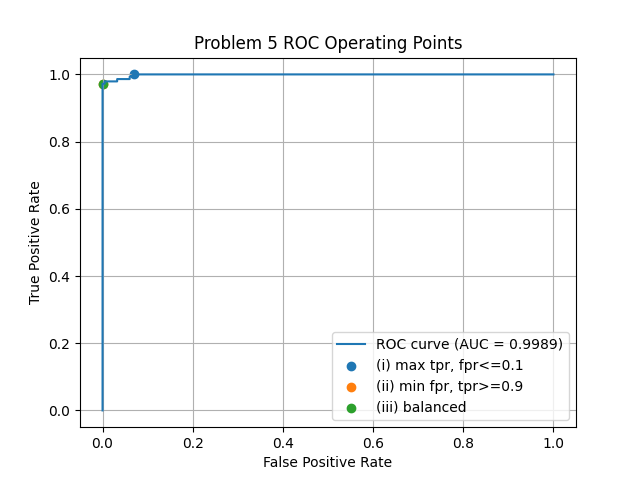
\includegraphics[width=0.5\textwidth]{plots/problem5_roc.png}
		\caption{Problem 5: ROC curve with selected operating points}
	\end{figure}
	
\end{document}